\chapter{Analisi del dominio e del contesto}
In questa sezione viene riportata la modellazione di classi e proprietà che compongono l'ontologia.


\section{Analisi del dominio}
Il dominio è inerente all'energia, in maniera specifica al Prosumer, ovvero un'entità che può sia produrre che consumare energia.
Un Prosumer è caratterizzato da:

\begin{itemize}
    \item Un profilo di carico equivalente o consumo;
    \item Un sistema di generazione;
    \item Un sistema di accumulo dell'energia o storage;
    \item Due o più contatori, detti anche punti di misura.
\end{itemize}

Un sistema di accumulo può essere monodirezionale, ovvero può assorbire energia elettrica solo dall’impianto di produzione, oppure bidirezionale, cioè può assorbire energia elettrica sia dall’impianto di produzione che dalla rete con obbligo di connessione di terzi.
Il principale elemento differenziante è quindi se lo storage assorbe energia esclusivamente dall’impianto di produzione.

In base alla configurazione (descritta in seguito), l'impianto può avere due o tre contatori:
\begin{itemize}
    \item Contatore M1: è il contatore di scambio con la rete di distribuzione, e misura l’energia scambiata (assorbita o immessa) con la rete.
    \item Contatore M2: è il contatore che misura l’energia scambiata nel punto di produzione (ovvero la combinazione dell’energia prodotta dal generatore con l’energia fornita o assorbita dal sistema di accumulo).
    \item Contatore M3: quando presente (configurazione 3 descritta più avanti), serve a misurare l’energia di carico e scarico del sistema di accumulo (tipicamente, una batteria elettrica).
\end{itemize}

È noto che il prosumer possa avere tre tipi di configurazioni, ovvero:
\begin{itemize}
    \item Configurazione 1:
          \begin{itemize}
              \item Sistema di accumulo monodirezionale, situato lato produzione e caratterizzato da corrente continua;
              \item Presenza dei contatori M1 e M2, assenza del contatore M3.
          \end{itemize}
    \item Configurazione 2:
          \begin{itemize}
              \item Sistema di accumulo bidirezionale, situazio lato produzione e caratterizzato da corrente che può essere sia alternata che continua;
              \item Presenza dei contatori M1, M2, assenza del contatore M3.
          \end{itemize}
    \item Configurazione 3:
          \begin{itemize}
              \item Sistema di accumulo bidirezionale, situato lato post-produzione e caratterizzato da corrente alternata;
              \item Presenza dei contatori M1, M2 e M3.
          \end{itemize}
\end{itemize}

\section{Classi}
L'ontologia è stata sviluppata focalizzandosi sul ruolo del prosumer e delle sue caratteristiche.
Di conseguenza è stato pensato di modellare come classi principali:
\begin{itemize}
    \item \textbf{Prosumer} per modellare l'individuo principale;
    \item Profilo di consumo, chiamato \textbf{Load}, per modellare la quantià di energia consumata;
    \item Sistema di generazione, chiamato \textbf{Generator}, per mdellare la quantià di energia prodotta;
    \item Sistema di accumulo, chiamato \textbf{Storage System}, composto da uno o più \textbf{Energy Storage} o \textbf{Battery}, per modellare l'energia immagazzinata;
    \item Contatore, chiamato \textbf{Energy Meter}, con sottoclassi \textbf{M1}, \textbf{M2} e \textbf{M3}, per modellare il controllo sulla quantità di energia scambiata all'interno di un prosumer;
    \item \textbf{Power Type}, con sottoclassi \textbf{AC} e \textbf{DC}, per modellare la tipologia di corrente;
    \item \textbf{Energy Storage Location}, con sottoclassi \textbf{Production} e \textbf{Post Production}, per modellare la posizione del sistema di accumulo;
    \item \textbf{Energy Direction}, con sottoclassi \textbf{Monodirectional} e \textbf{Bidirectional}, per modellare la direzione del sistema di accumulo.
\end{itemize}

Per quanto riguarda la modellazione di \textbf{Storage System} e di \textbf{Battery}, è stata utilizzata l'ontologia \textit{Battery} sviluppata da Kyrillos.

Le varie configurazioni sono state modellate come sottoclassi di \textbf{Prosumer}, ovvero \textbf{Config01}, \textbf{Config02} e \textbf{Config03}.
A seconda delle equivalenze dichiarate all'interno di ogni sottoclasse di \textbf{Configuration}, sarà il reasoner a dichiarare a che configurazione appartengono le istanze di tipo Prosumer.

Le varie sottoclassi sono tutte disgiunte tra loro, in quanto ritenuto concettualmente non possibile l'appartenenza di un'istanza a più classi diverse.
Anche le classi principali come \textit{Load}, \textit{Generator} e altre sono disgiunte tra loro per la stessa motivazione.

In seguito si può vedere la struttura dell'ontologia, con le classi principali e le loro sottoclassi, compresa di estensioni quali \textit{SAREF}, \textit{InterConnect} e \textit{Battery}.

\begin{figure}[!ht]
    \centering
    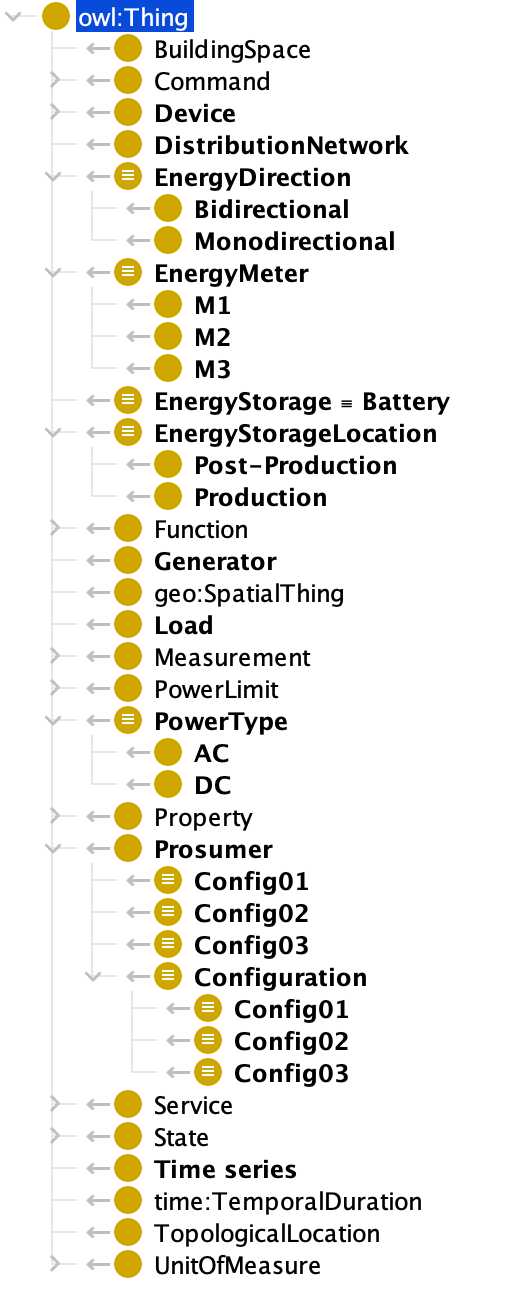
\includegraphics[width=7cm]{images/classi_prosumer.png}
    \caption{Struttura dell'ontologia Prosumer.}
    \label{fig:classi_prosumer}
\end{figure}


\section{Proprietà}

\section{Data Properties}